 \documentclass[11pt,a4paper,onecolumn]{article}

% !TeX root = ./Sup_info.tex
\setlength{\columnsep}{1cm}
 

\usepackage[T1]{fontenc}       % Use modern font encodings
% \usepackage[version=3]{mhchem} % Formula subscripts using \ce{}
\usepackage{graphicx}
\usepackage[a4paper,top=2cm, bottom=2.5cm, left=2.5cm, right=2.5cm]{geometry}
% \usepackage{authblk} % For affiliation. This package is not preinstalled.
\graphicspath{{Figure_SI/}}
\usepackage{xr} 
\externaldocument{azurin} 

\newcommand*\commentauthor[1]{\textbf{{\textit{#1}}}}
\newcommand*\me[1]{\ensuremath{\bar{#1}\,}}
\newcommand*\chem[1]{\ensuremath{\mathrm{#1}}}
\newcommand*{\affaddr}[1]{#1} % No op here. Customize it for different styles.
\newcommand*{\affmark}[1][*]{\textsuperscript{#1}}
\newcommand*{\email}[1]{\texttt{#1}} % These three commands are for author affilations.

\linespread{1.3} % Line spacing. 1.3 means one-and-a-half spacing.

\begin{document}

\author{Authors
%Biswajit Pradhan, Sebastiaan Van Mulken, Xueyan Miao, Gerard Canters, Michel Orrit\\\affaddr{Huygens-Kamerlingh Onnes Laboratory, Leiden University, 2300 RA Leiden, Netherlands}\\\email{orrit@physics.leidenuniv.nl}
}

\date{\vspace{1ex}} % Exclude date in the title.

\title{\textbf{Single azurin redox switching}\\ \vspace{3ex} Supplementary Information \vspace{3ex}}

\maketitle
\tableofcontents
\pagebreak
%=====================METHODS AND FIGURES===========================
% \section{Protein and labeling}
%Peak separation
\begin{figure}
  \centering
  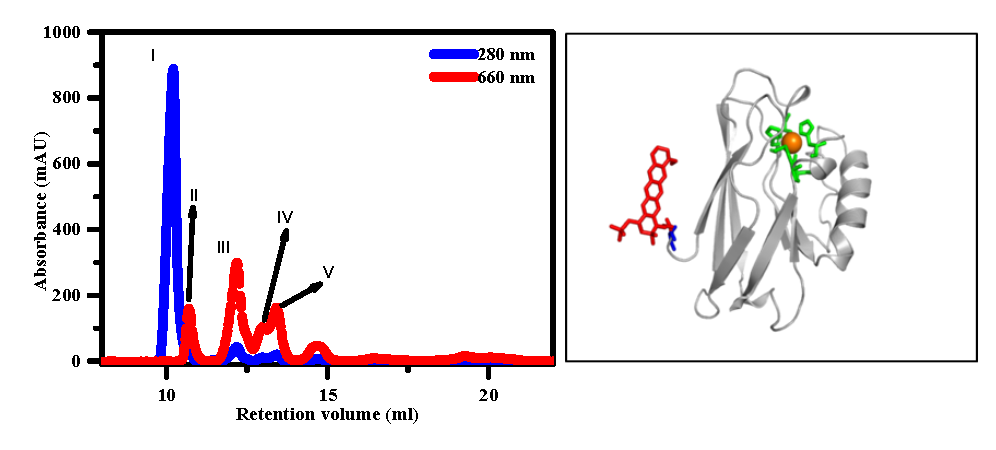
\includegraphics[width=0.8\textwidth]{peak_separation.eps}
  \makeatletter
  \renewcommand{\fnum@figure}{\figurename~S\thefigure}
  \makeatother
  \caption{Peak separation: (a) Elution profile of Cu azurin sample after labeling and removal of free dye. 280 nm absorption that tells the presence of protein is shown in blue and 660 nm absrption that tells the presence of dye is shown in red. The protein structure with the dye at Lys 122 corresponding to peak-III is shown in the right. {A proper structure will be replaced}}
  \label{SIfig: peak_sep}
\end{figure}
% \pagebreak
\section{Fluorescence switching in bulk}
%BULK Switching
Fluorescence measurements in bulk of different peaks of azurin-ATTO655 sample (Figure S\ref{SIfig: peak_sep}) were carried out to determine the FRET switching ratio. The measurements were done in Cary Eclipse Spectrometer (Varian Inc. Agilent Technology, USA). A 50 nM sample was excited with 665 nm and intensity was monitored above 675 nm. Sodium ascorbate (reductant) and Pottasium ferrocyanide (oxidant) were added alternatively. Among all the labeled position, peak-III showed maximum switching ratio and it's intensity change can be seen in Figure S\ref{SIfig: switching}. Similarly Zn Azurin-ATTO655 showed little or no change in intensity.
\begin{figure}
  \centering
  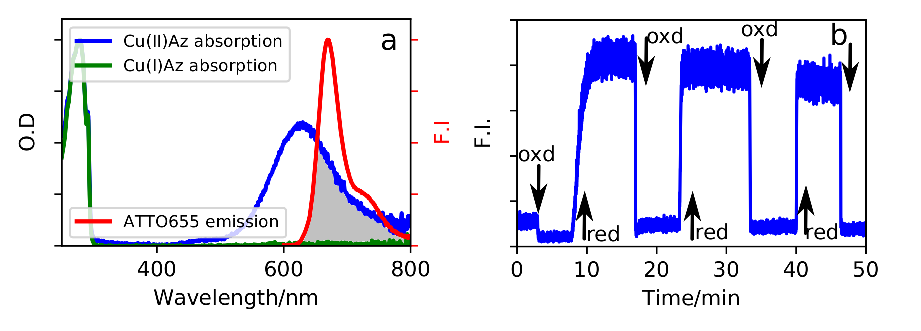
\includegraphics{spectral_overlap_switching.eps}
  \makeatletter
  \renewcommand{\fnum@figure}{\figurename~S\thefigure}
  \makeatother
  \caption{Spectral overlap and Bulk switching: (a) Absorption spectrum of Cu(II)azurin (blue), Cu(I)azurin (black). The emission spectrum of ATTO655 (red) has a good overlap with the absorption of Cu(II)azurin to show high FRET. (b) Fluorescence intensity of 50 nM CuAzurin-ATTO655 shows high intensity in the presence of reductant and low intensity with oxidant. The switching ratio comes to be 90\% satisfying the requirement for single-molecule FRET.}
  \label{SIfig: switching}
\end{figure}
%time trace Zn and Cu azurin
\begin{figure}
  \centering
  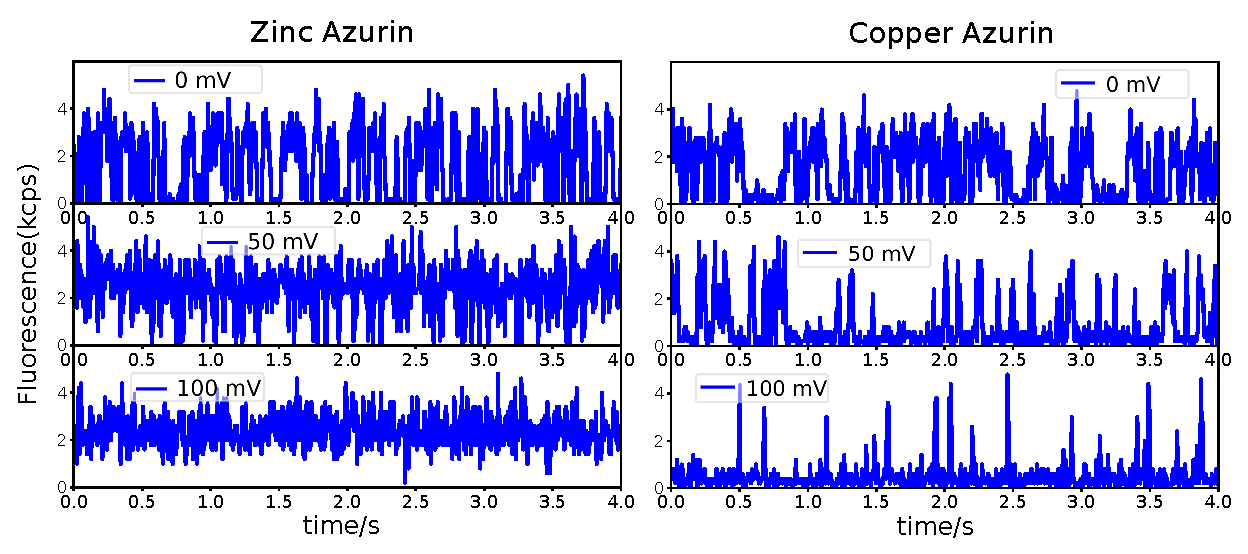
\includegraphics[width=\textwidth,keepaspectratio]{SI_timetrace_Zn_Cu.eps}
  \makeatletter
  \renewcommand{\fnum@figure}{\figurename~S\thefigure}
  \makeatother
  \caption{Time traces of Zn Azurin (left) and of Cu Azurin(right) labeled with ATTO655 at different potential.  Above 25 mV, Cu-Azurin show swiching in the intensity due to changes in the oxidation state of the Copper metal center and below 25 mV, triplet blinking contributes to the switching as can be seen in the redox inactive Zn-Azurin. To keep the analysis simple, time traces above 40 mV were choosen for Cu azurin}
  \label{SIfig:tracecomparision}
\end{figure}
%lifetime and switching ration from time trace
\begin{figure}
  \centering
  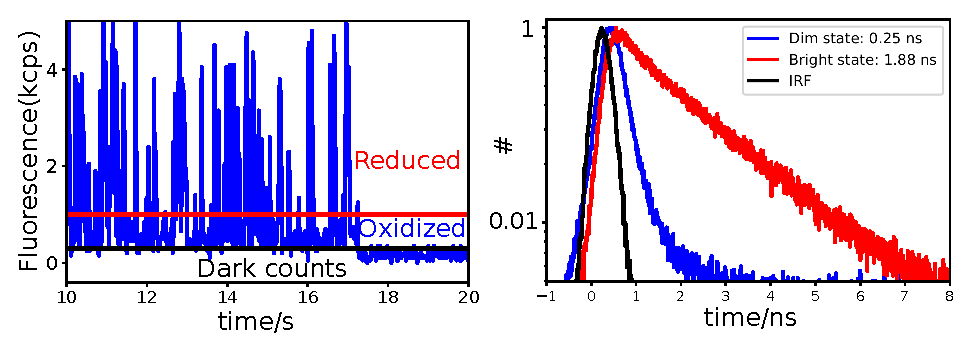
\includegraphics{lifetime.eps}
  \makeatletter
  \renewcommand{\fnum@figure}{\figurename~S\thefigure
}  \makeatother
  \caption{Single-molecule azurin switching and lifetime. (a) Time trace of a single Cu azurin at 50 mV with a binning time of 50 ms. Notice the three different label indicated in the figure. Bright (Cu(I)) state as above the red line, oxidized state is between red and black and Dark counts are below the black line. The fact that the molecule doesn't go to the dark count label before being bleached shows that the transitions are due to Copper oxidation switching rather than triplet blinking of the dye. Once the fluorophore is bleached, no transitions were observavable. (b) The lifetime histogram corresponding to bright state (red), oxidized state (blue) and instrument response function (black). The lifetime of oxidized state is much shorter than the reduced state due to FRET quenching.}
  \label{SIfig: lifetime}
\end{figure}
%FCS comparision
\begin{figure}
  \centering
  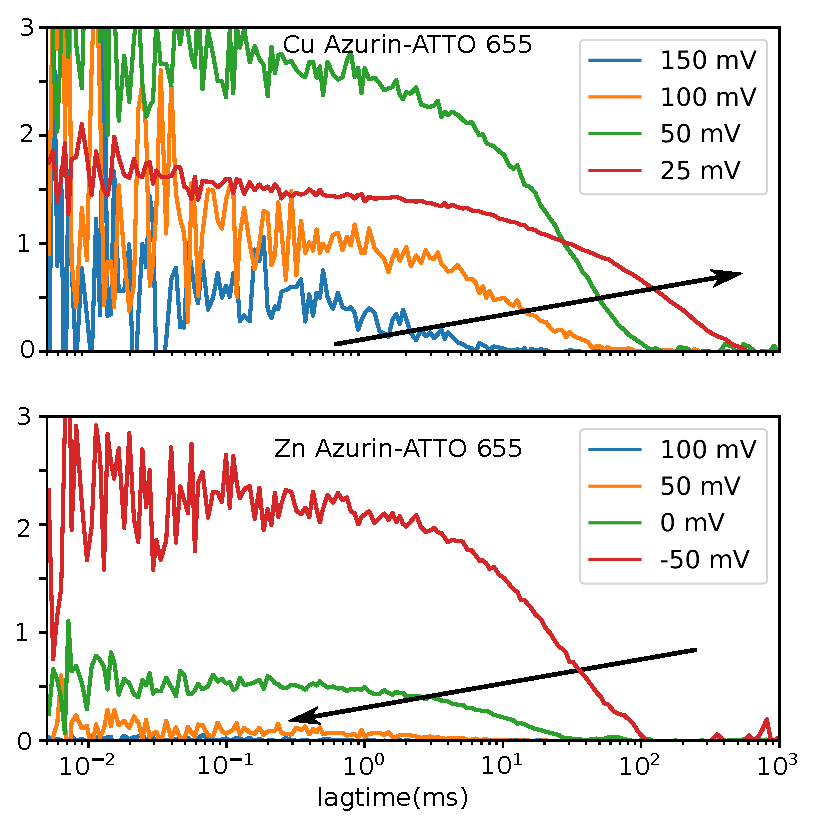
\includegraphics[]{fcs_comparision.eps}
  \makeatletter
  \renewcommand{\fnum@figure}{\figurename~S\thefigure}
  \makeatother
  \caption{Autocorrelation of time traces of Cuazurin-ATTO655 (a) and Znazurin-ATTO655 at different potential. At lower potential, Cuazurin-ATTO655 has longer correlation time (on time) which shows that the molecule spends more time on the Cu(I) state. But below 50 mV the dye (ATTO655) starts to show triplet blinking. As potential is lowered the triplet blinking dominates. The Cu azurin study is focussed in the safe window of potential more than 40 mV where triplet blinking is absent.}
  \label{SIfig:fcscomparision}
\end{figure}
%Slope: Nernst equation
\begin{figure}
  \centering
  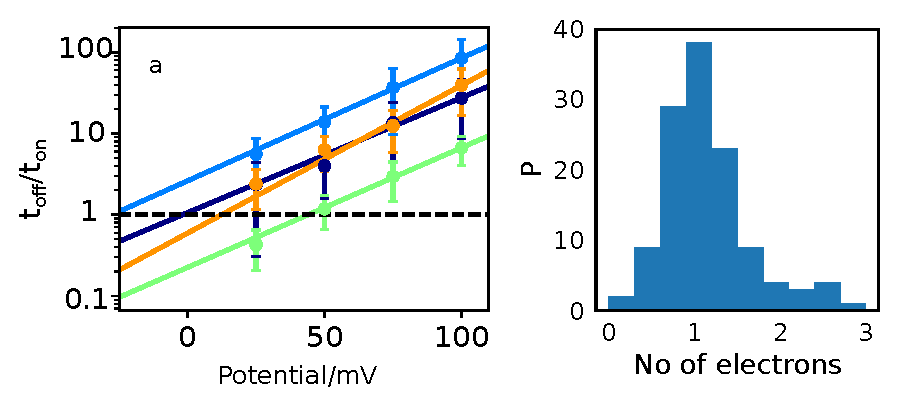
\includegraphics[width=\textwidth,keepaspectratio]{SI_potential_slope.eps}
	\makeatletter
	\renewcommand{\fnum@figure}{\figurename~S\thefigure}
	\makeatother
  \caption{Fitting with Nernst equation with slope as variable parameters for  (a) Cu-Azurin ATTO655. (b) The corresponding histogram of slopes obtained from the fitting shown in the left. the distribution of slope is centered around $59~$mV indicating that Cuazurin switching  involves only one electron.}
  \label{SIfig:potential_slope}
\end{figure}
%Rate fit at all potential
\begin{figure}
  \centering
  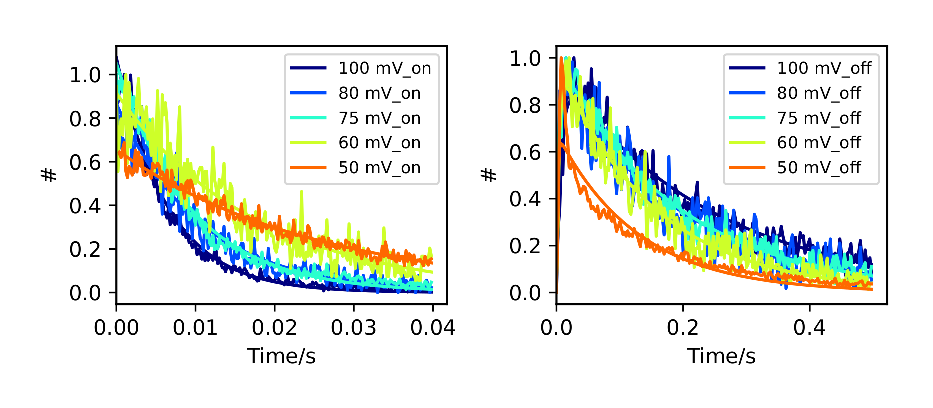
\includegraphics{rate_fit_all_potential.eps}
  \makeatletter
  \renewcommand{\fnum@figure}{\figurename~S\thefigure}
  \makeatother
  \caption{(a) Fitting of $on$ time distribution with monoexponential at different potential. (a) Fitting of $off$ time distribution with bi-exponential equation with rise time as shown in the main text at different potential. the output rate constants were plotted against potential (see main text)}
  \label{SIfig: rate_fit_all_potential}
\end{figure}
%No of averaging points
\begin{figure}
  \centering
  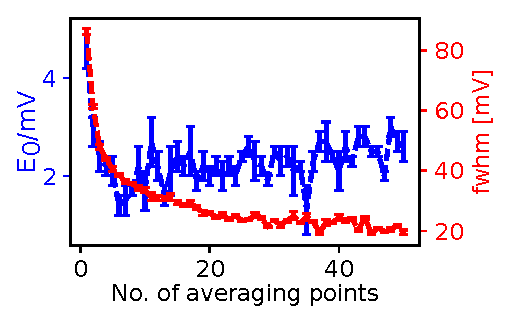
\includegraphics[scale=1.5]{N_avgpoints_vs_fwhmwidth.eps}
  \makeatletter
  \renewcommand{\fnum@figure}{\figurename~S\thefigure}
  \makeatother
  \caption{Variation of midpoint potential and fwhm with the number of on and off times taken for averaging for the long trace shown in the main text (Figure-\ref{fig:long_azurin_trace}). At around $20~$ events, both $E_0$ and fwhm reaches palteu. The averaging of on-time and off-times for correlation and midpoint distribution were done every $20$ events.}
  \label{SIfig: N_avgpoints_vs_fwhmwidth}
\end{figure}
% \pagebreak
% \bibliographystyle{ieeetr} % For a list of bibliography styles, see https://www.sharelatex.com/learn/Bibtex_bibliography_styles
% \bibliography{Sup_info}
\end{document}